\documentclass[../../index.tex]{subfiles}

\begin{document}
\chapter{$\tau$ decays into hadrons}
\begin{equation}
  R_\tau = \frac{\Gamma(\tau \to \nu_\tau + \text{Hadrons})}{\Gamma(\tau \to \nu_\tau e^+ e^-)}
\end{equation}

in terms of V/A, S/P \cite{Broadhurst1975}
\begin{equation}
  \begin{split}
    \Pi^{\mu\nu}(q^2) &= (q^\mu q^\nu - q^2 g^{\mu\nu}) \Pi^{V,A}(q^2) + \frac{g^{\mu\nu}}{q^2} (m_i \mp m_j)\Pi^{S,P}(q^2) \\
    &+ g^{\mu\nu}\frac{(m_i \mp m_j)}{q^2} [ \langle \anti{q}_i q_i \rangle \mp \langle \anti{q}_j q_j \rangle]
  \end{split}
\end{equation}

\begin{equation}
  q_\mu q_\nu \Pi^{\mu\nu}(q^2) = (m_i \mp m_j)^2 \Pi^{S,P}(q^2) + (m_i \mp m_j)[\langle \anti{q}_i q_i \rangle \mp \langle \anti{q}_j q_j \rangle]
\end{equation}

in terms of T and L
\begin{equation}
  \Pi^{\mu\nu}(q^2) = (q^\mu q^\nu - g^{\mu\nu}q^2) \Pi^{(T)}(q^2) + q^\mu q^\nu \Pi^{(L)}(q^2)
\end{equation}

\begin{equation}
  q_\mu q_\nu \Pi^{\mu\nu}(q^2) = q^4 \Pi^{(L)}(q^2) = s^2 \Pi^{(L)}(s),
\end{equation}
where $s \equiv q^2$

relation L and S,P
\begin{equation}
  s^2 \Pi^{(L)}(s) = (m_i \mp m_j)^2 \Pi^{(S,P)}(s) + (m_i \mp m_j)[ \langle \anti{q}_i q_i \rangle \mp \langle \anti{q}_j q_j \rangle]
\end{equation}

need relation T and V,A
\begin{equation}
  \label{eq:longitudinalCorrelator}
  \begin{split}
    \Pi^{\mu\nu}(s) &= \underbrace{(q^\mu q^\nu - g^{\mu\nu}q^2)\Pi^{(T)}(s) + (q^\mu q^\nu - g^{\mu\nu} q^2)\Pi^{(L)}(s)}_{=(q^\mu q^\nu - g^{\mu\nu} q^2) \Pi^{(T+L)}(s)} + \frac{g^{\mu\nu}s^2}{q^2}\Pi^{(L)}(s)
  \end{split} 
\end{equation}
where $\Pi^{(T+L)}(s) \equiv \Pi^{(T)}(s) + \Pi^{(L)}(s)$
\begin{equation}
  \Pi^{(V,A)}(s) = \Pi^{(T)}(s) + \Pi^{(L)} = \Pi^{(T+L)}
\end{equation}

\begin{equation}
  q_\mu q_nu
\end{equation}

The theoretical expression of the hadronic $\tau$-decay ratio was first derived
by \cite{Tsai1971} (using current algebra, a more recent derivation making use
of the *optical theorem* can be taken from \cite{Schwab2002}):
\begin{equation}
  \label{eq:hadronicTauDecayRatio}
  R_\tau = 12 \pi \int_0^{m_\tau} = \frac{\dif s}{m_\tau^2}
  \left( 1 - \frac{s}{m_\tau^2} \right)
  \left[ \left( 1 + 2 \frac{s}{m_\tau^2} \right) \Ima \Pi^{(T)}(s) + \Ima \Pi^{(L)} \right].
\end{equation}
$R_\tau$ introduces a problematic integral over the real axis of $\Pi(s)$ from $0$ up to
$m_\tau$. The integral is problematic for two reasons:
\begin{itemize}
  \item The \textit{perturbative Quantum Chromodynamcs} (\textbf{pQCD}) and the OPE breaks down for low
    energies (over which we have to integrate).
  \item The positive euclidean axis of $\Pi(s)$ has a discontinuity cut and can
    theoretically not be evaluated.
\end{itemize}
To literally circunvent these issues we make use of \textit{Cauchy's Theorem}
\begin{equation}
  \int_{\mathcal{C}} f(z) \dif z = 0,
\end{equation}
where $f(z)$ is an analytic function on a closed contour $\mathcal{C}$.

In our case we have to deal with the two-point correlator $\Pi(s)$, which is analytic
except for the positive real axis (with which we will deal with to a later
point\footnote{To not evaluate $\Pi(s)$ at the positive real axis we have to
  introduce \textit{pinched weights}. The \textit{pinched weights} vanish for $s
  \to m_\tau$.}) Consequently, to rewrite we can rewrite the definite integral of
\cref{eq:hadronicTauDecayRatio} into a contour integral over a closed circle
with
radius $m_\tau^2$. The closed contour consists of four line integrals,
which have been visualized in \cref{fig:rTauCauchysTheorem}. Summing over the
four line integrals, performing a \textit{analytic continuation} of the
two-point correlator $\Pi(s) \to \Pi(s + i \epsilon)$ and finally taking the
limit of $\epsilon \to 0$ gives us the needed relation between
\cref{eq:hadronicTauDecayRatio} and the closed contour:
\begin{equation}
  \begin{split}
  \oint_{s=m_\tau} \Pi(s) &= \int_0^{m_\tau} \Pi(s + i \epsilon) + \int_{\mathcal{C}_2}\Pi(s) \dif s + \int_{m_\tau}^0 \Pi(s - i \epsilon) \dif s + \int_{\mathcal{C}_4} \Pi(s) \dif s \\
  &= \int_0^{m_\tau} \Pi(s+i \epsilon) - \Pi(s - i \epsilon) \dif s  + \int_{\mathcal{C}_2}\Pi(s) \dif s + \int_{\mathcal{C}_4} \Pi(s) \dif s \\
  &= \int_0^{m_\tau} \Pi(s + i \epsilon) - \overline{\Pi(s + i \epsilon)} + \int_{\mathcal{C}_2}\Pi(s) \dif s + \int_{\mathcal{C}_4} \Pi(s) \dif s \\
  &\overset{\lim \epsilon \to 0}{=} 2 i \int_0^{m_\tau} \Ima \Pi(s) \dif s + \oint_{s=m_\tau} \Pi(s) \dif s
  \end{split}
\end{equation}
where we made use of $\Pi(z) = \overline{\Pi(\overline z)}$ (due to $\Pi(s)$ is analytic) and
$\Pi(z) - \overline{\Pi(z)} = 2 i \Ima \Pi(z)$. The result can be rewritten in a
more intuitive form, which we also visualized in \cref{fig:rTauCauchysTheorem}
\begin{equation}
  \label{eq:correlatorContourIntegral}
  \int_0^{m_\tau} \Pi(s) \dif s = \frac{i}{2} \oint_{s=m_\tau} \Pi(s) \dif s
\end{equation}
\begin{figure}
  \centering
  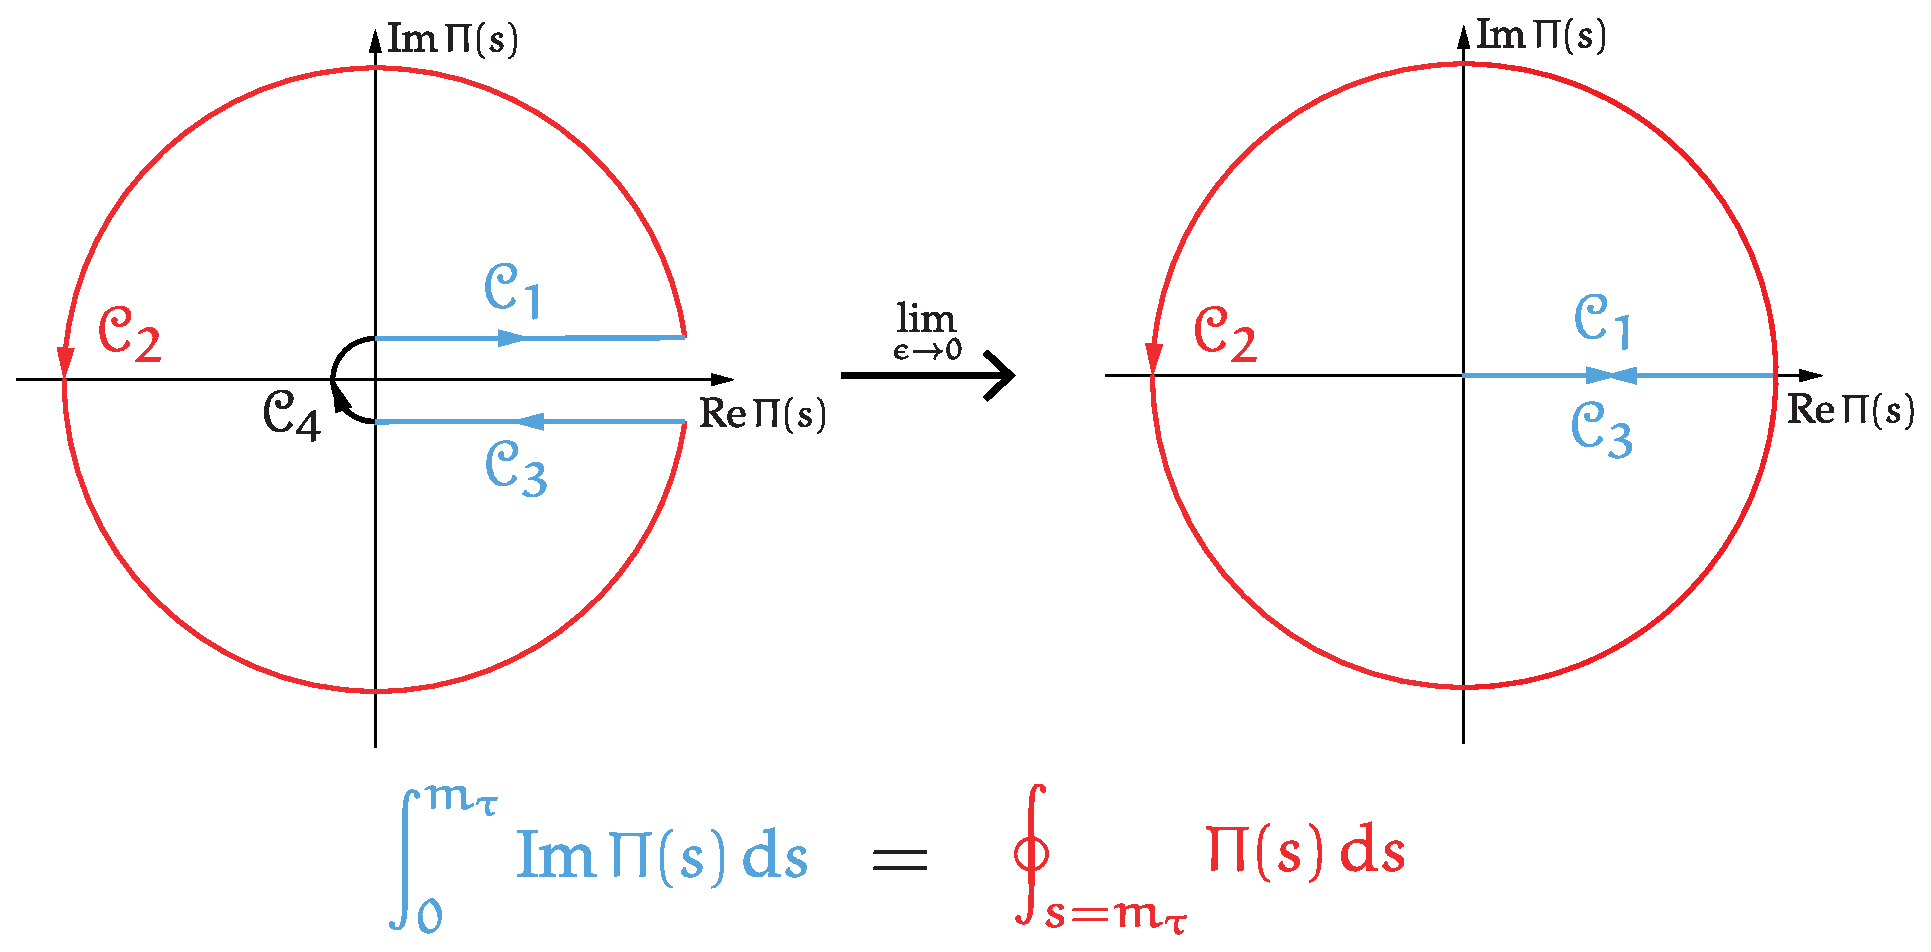
\includegraphics[width=0.8\textwidth]{./images/rTauCauchysTheorem.eps}
  \caption{Visualization of the usage of Cauchy's theorem to transform
    \cref{eq:hadronicTauDecayRatio} into a closed contour integral over a circle
  of radius $m_\tau^2$.}
  \label{fig:rTauCauchysTheorem}
\end{figure}
Finally combining \cref{eq:correlatorContourIntegral} with
\cref{eq:hadronicTauDecayRatio} we get
\begin{equation}
  R_\tau = 6 \pi i \oint_{s=m_\tau} \frac{\dif s}{m_\tau^2}
  \left( 1 - \frac{s}{m_\tau^2} \right)
  \left[ \left( 1 + 2 \frac{s}{m_\tau^2} \right) \Pi^{(T)}(s) + \Pi^{(L)} \right]
\end{equation}
for the hadronic $\tau$-decay ratio.

The contour integral obtained is an import result as we can now theoretically
evaluate the hadronic $\tau$-decay ratio sufficiently large energy scales
($m_\tau \approx \SI{1.78}{\mega\electronvolt}$) at which
$\alpha_s(m_\tau)\approx 0.33$ \cite{Pich2016} is tolerable heigh for applying
perturbation theory and the OPE. Obviously we would benefit from a contour integral over a
bigger circunference, but $\tau$-decays are limited by the $m_\tau$.
Nevertheless there are promising $e^+e^-$ annihilation data, which yields
valuable R-ratio values up to $\SI{2}{\giga\electronvolt}$
\cite{Boito2018}\cite{Keshavarzi2018}.

It is convenient to rewrite the 

\begin{equation}
  \Pi^{(L+T)} = \Pi^{(L)} + \Pi^{(T)}
\end{equation}

\begin{equation}
  R_\tau = 6 \pi i \oint_{\abs{s}=m_\tau} \frac{\dif s}{m_\tau^2} \left( 1 - \frac{s}{m_\tau^2} \right)^2 \left[ \left( 1 + 2 \frac{s}{m_\tau^2} \right) \Pi^{(L+T)}(s) - \left( \frac{2 s}{m_\tau^2} \right) \Pi^{(L)}(s) \right]
\end{equation}
\begin{equation}
  \label{eq:adlerFunction}
  D^{(L+T)}(s) \equiv -s \od{}{s} \Pi^{(L+T)}(s), \qquad D^{(L)}(s) \equiv \frac{s}{m_\tau^2} \od{}{s} (s \Pi^{(L)}(s))
\end{equation}
Integration by parts
\begin{equation}
  \int_a^b u(x) V(x) \dif x = \left[ U(x) V(x) \right]_a^b - \int_a^b U(x) v(x) \dif x
\end{equation}
\begin{equation}
  \begin{split}
    R_\tau^{(1)} &= \frac{6 \pi i}{m_\tau^2} \oint_{\abs{s}=m_\tau^2}\underbrace{\left( 1 - \frac{s}{m_\tau^2} \right)^2 \left( 1 + 2 \frac{s}{m_\tau^2} \right)}_{=u(x)} \underbrace{ \vphantom{\left( \frac{s}{m_\tau^2} \right)} \Pi^{(L+T)}(s)}_{=V(x)} \\
    &= \frac{6 \pi i}{m_\tau^2} \left\{  \left[ -\frac{m_\tau^2}{2} \left( 1 - \frac{s}{m_\tau^2} \right)^3 \left( 1 + \frac{s}{m_\tau^2} \right) \Pi^{(L+T)}(s) \right]_{\abs{s}=m_\tau^2} \right. \\
    &\quad+ \oint_{\abs{s}=m_\tau^2} \underbrace{-\frac{m_\tau^2}{2} \left( 1 - \frac{s}{m_\tau^2} \right)^3 \left( 1 + \frac{s}{m_\tau^2} \right)}_{=U(x)} \underbrace{\vphantom{\left( \frac{1}{m_\tau^2} \right)}\od{}{s} \Pi^{(L+T)}(s)}_{=v(x)} \left. \vphantom{\left[ \left( \frac{1}{m_\tau^2} \right) \right]} \right\} \\
    &= -3 \pi i \oint_{\abs{s}=m_\tau^2s} \frac{\dif s}{s} \left( 1 - \frac{s}{m_\tau^2} \right)^3 \left( 1 + \frac{s}{m_\tau^2} \right) \od{}{s} D^{(L+T)}
  \end{split}
\end{equation}
where we fixed the integration constant to $C=-\frac{m_\tau^2}{2}$ in the second
line and left the antiderivatives contained in the squared brackets untouched.
Parametrizing the expression in the squared brackets
\begin{equation}
    \left[ -\frac{m_\tau^2}{2} \left( 1 - e^{-i \phi} \right)^3 \left( 1 + e^{-i \phi} \right) \Pi^{(L+T)}(m_\tau^2 e^{-i \phi}) \right]_0^{2\pi} = 0
\end{equation}
where $s \to m_\tau^2 e^{-i \phi}$ and $(1 - e^{-i \cdot 0}) = (1 - e^{-i \cdot 2 \pi})
= 0$.

\begin{equation}
  \begin{split}
    R_\tau^{(2)} &= \oint_{\abs{s}=m_\tau^2} \dif s \left( 1 - \frac{s}{m_\tau^2} \right)^2 \left( - \frac{2 s}{m_\tau^2} \right) \Pi^{(L)}(s) \\
    &= - 4 \pi i \oint \frac{\dif s}{s} \left( 1 - \frac{s}{m_\tau^2} \right)^3 D^{(L)}(s)
  \end{split}
\end{equation}

\begin{equation}
  R_\tau = - \pi i \oint_{\abs{s}=m_\tau^2} \frac{\dif s}{s} \left( 1 - \frac{s}{m_\tau^2} \right)^3 \left[ 3 \left( 1 + \frac{s}{m_\tau^2} D^{(L+T)}(s) + 4 D^{(L)}(s) \right) \right]
\end{equation}

\begin{equation}
  \label{eq:rTauFinal}
  R_\tau = - \pi i \oint_{\abs{s}=m_\tau^2} \frac{\dif x}{x} (1 - x)^3 \left[ 3 (1 + x) D^{(L+T)}(m_\tau^2 x) + 4 D^{(L)}(m_\tau^2 x)  \right],
\end{equation}
where $x=s/m_\tau^2$.

\begin{equation}
  \label{eq:rTauContributions}
  R_{\tau,V/A}^\omega = \frac{N_c}{2}S_{EW} \abs{V_{ud}}^2 \left( 1 + \delta_{\omega}^{(0)} + \delta^{EW}_{\omega} + \delta_{\omega}^{DVs} + \sum_{D \leq 2} \delta^{(D)}_{ud,\omega} \right)
\end{equation}

\section{The perturbative expansion}
We will treat the correlator in the chiral limit for which the longitudinal
components $\Pi^{L}(s)$ vanish (see \cref{eq:longitudinalCorrelator}) and the
axial and vectorial contributions are equal. Consequently \cite{Beneke2008} we
can write the vector correlation function $\Pi(s)$ as:
\begin{equation}
  \label{eq:correlatorExpansion}
  \Pi_V^{T+L}(s) = - \frac{N_c}{12 \pi^2} \sum_{n=0}^\infty a_\mu^n \sum_{k=0}^{n+1} c_{n,k} L^{k} \quad \text{with} \quad L \equiv \ln \frac{-s}{\mu^2}.
\end{equation}

The coeffiecient $c_{n,k}$ up to two-loop order can be
obtained by Feynman-diagram calculations.
\textcolor{red}{add complete calculation}
E.g. we can compare the zero-loop result of the correlator \cite{Jamin2006}
\begin{equation}
  \left. \Pi^B_{\mu\nu}(q^2) \right\rvert^{1-loop} = \frac{N_c}{12\pi^2} \left( \frac{1}{\hat \epsilon} - \log\frac{(-q^2 - i0)}{\mu^2} + \frac{5}{3} + \mathcal{O}(\epsilon) \right)
\end{equation}
with \cref{eq:correlatorExpansion} and extract the first two coefficients 
\begin{equation}
  c_{00} = - \frac{5}{3} \qquad \text{and} \qquad c_{01} = 1,
\end{equation}
where $\Pi^B_{\mu\nu}(q^2)$ is not renormalized\footnote{The term $1/ \hat
  \epsilon$, which is of order 0 in $\alpha_s$, will be cancelled by renormalization.}

The second loop can also be calculated by diagram techniques resulting in \cite{Boito2011}
\begin{equation}
  \left. \Pi_V^{(1+0)}(s) \right\rvert^{2-loop} = -\frac{N_c}{12\pi^2} a_\mu \log(\frac{-s}{\mu^2}) + \cdots
\end{equation}
yielding  $c_{11} = 1$.

Beginning from three loop diagrams the algebra becomes exausting and one has to
use dedicated algorithms to compute the heigher loops. The third loop
calculations have been done in the late seventies by
\cite{Chetyrkin1979,Dine1979,Celmaster1979}. The four loop evaluation have been
completed a little more than ten years later by
\cite{Gorishnii1990,Surguladze1990}. The heighest loop published, that amounts
to $\alpha_s^4$, was published in 2008 \cite{Baikov2008} almost 20 years later.

Fixing the number of colors to $N_c=3$ the missing coefficients up to order four
in $\alpha_s$ read:
\begin{equation}
  \begin{split}
    c_{2,1} &= \frac{365}{24} - 11 \zeta_3 - \left( \frac{11}{12} - \frac{2}{3}\zeta_3 \right) N_f \\ 
    c_{3,1} &= \frac{87029}{288} - \frac{1103}{4} \zeta_3 + \frac{275}{6}\zeta_5 \\
           &- \left( \frac{7847}{216} - \frac{262}{9} \zeta_3 + \frac{25}{9} \zeta_5 \right) N_f + \left( \frac{151}{162} - \frac{19}{27}\zeta_3\right)N_f^2 \\
   c_{4,1} &= \frac{78631453}{20736} - \frac{1704247}{432}\zeta_3 + \frac{4185}{8}\zeta_3^2 + \frac{34165}{96}\zeta_5 - \frac{1995}{16}\zeta_7,
  \end{split}
\end{equation}
where used the flavour number $N_f=3$ for the last line.

The 6-loop calculation has until today not been achieved, but Beneke und Jamin
\cite{Beneke2008} used and educated guess to estimate the coefficient
\begin{equation}
  c_{5,1} \approx 283 \pm 283.
\end{equation}

Until know we have mentioned the coefficients $c_{n,k}$ with a fixed $k=1$. This
is due to the RGE, which relates coefficients with a different $k$ to the
coefficients mentioned above. To make usage of the RGE $\Pi_V^{T+L}(s)$ needs to
be a physical quantity, which can be achieved by rewriting \cref{eq:adlerFunction} to:
\begin{equation}
  D_V^{(T+L)} = - s \od{\Pi_V^{(T+L)}(s)}{s} = \frac{N_c}{12 \pi^2} \sum_{n=0}^\infty a_\mu^n \sum_{k=1}^{n+1} k c_{n,k} L^{k-1},
\end{equation}
where we used $\dif L^k/ \dif s=k\ln(-s/\mu^2)^{k-1}(-1/\mu^2)$. $D_V^{1+0}$
being a physical quantity has to fulfill the RGE \cref{eq:RGE}
\begin{equation}
  -\mu \od{}{\mu} D_V^{(T+L)} = -\mu \od{}{\mu} \left( \pd{}{L} \dif L + \pd{}{a_s} \dif a_s \right) D_V^{T+L}
  = \left( 2\pd{}{L} + \beta \pd{}{a_s} \right) D_V^{T+L} = 0,
\end{equation}
where we defined the $\beta$-function in \cref{eq:betaFunction} and used $\dif L
/ \dif \mu = - 2/ \mu$. The RGE puts constraints on the $c_{n, k}$-coefficients,
... not independent
\begin{equation}
  D(s) = \frac{N_c}{12 \pi^2} \left[ c_{01} + a_\mu(c_{11} + 2 c_{12} L) + a_\mu^2(c_{21} + 2 c_{22} L + 3 c_{23} L^2) \right]
\end{equation}
inserting into RGE
\begin{equation}
  4 a_\mu c_{12} + 2 a_\mu^2(2 c_{22} + 6 c_{23} L) + \beta_1 a_\mu^2(c_{11} + 2 c_{12}L) + \mathcal{O}(a_\mu^3) = 0
\end{equation}
Thus
\begin{equation}
  c_{12} = 0 \quad c_{22} = \frac{\beta_1 c_{11}}{4} \quad c_{23} = 0
\end{equation}
or $D(s)$ to the first order in $\alpha_s$
\begin{equation}
  D(s) = \frac{N_c}{12 \pi^2} \left[ c_{01} + c_{11} a_\mu \left( c_{21} - \frac{1}{2} \beta_1 c_{11} L  \right) a_\mu^2 \right] + \mathcal{O}(a_\mu^3)
\end{equation}

\subsection{Renormalisation group summation}
We can express the perturbative contribution $\delta^{(0)}$ to $R_\tau$ (see
\cref{eq:rTauContributions}) as
\begin{equation}
  \label{eq:rTauDelta0}
  \delta^{(0)} = \sum_{n=1}^{\infty} a_\mu^n \sum_{k=1}^n k c_{n,k} \frac{1}{2 \pi i} \oint_{\abs{x}=1} \frac{\dif x}{x} (1-x)^3(1+x) \log \left( \frac{-M_\tau^2 x}{\mu^2} \right)^{k-1},
\end{equation}
where we inserted the expansion of $D_V^{(T+L)}$ \cref{eq:adlerFunction} into
$R_\tau$ \cref{eq:rTauFinal}. Keep in
mind that we are working in the chiral limit, such that $D^{L}=0$ vanishes and
the contributions from the vector and axialvector correlator are identical
\begin{equation}
  D^{(T+L)} = D^{(T+L)}_V + D^{(T+L)}_A = 2 D^{(T+L)}_V.
\end{equation}

The perturbative contribution $\delta^{(0)}$ is a physical quantity and
satisfies the homogeneous RGE, thus is independent on the scale $\mu$.
Consequently we have the freedom to choose $\mu$, which leads to two main
descriptions \textbf{fixed-order perturbation theory} (FOPT) and
\textbf{contour-improved perturbation theory} (CIPT). The two resulting series
should converge to equal values, but differ notably. 


By using the FOPT prescription we fix $\mu^2=m_\tau^2$ leading to
\begin{equation}
  \delta_{FO}^{(0)} = \sum_{n=1}^\infty a(m_\tau^2)^n \sum_{k=1}^n k c_{n,k} J_{k-1}
\end{equation}
where the contour integrals $J_l$ are defined by
\begin{equation}
  J_l \equiv \frac{1}{2\pi i} \oint_{\abs{x}=1} \frac{\dif x}{x} (1-x)^3(1+x) \log^l(-x).
\end{equation}
The integrals $J_l$ up to order $\alpha_s^4$ are given by \cite{Beneke2008}:
\begin{equation}
  J_0 = 1, \quad J_1 = -\frac{19}{12} \quad J_2 = \frac{265}{72} - \frac{1}{3} \pi^2, \quad J_3 = - \frac{3355}{288} + \frac{19}{12}\pi^2.
\end{equation}
Using FOPT the strong coupling $a(\mu)$, which runs with the scale $\mu$, is
fixed at $a(m_\tau^2)$ and can be taken out of the closed-contour integral. We
still have to integrate over the logarithms $\log(-s/m_\tau^2)$. 

Using CIPT we can sum the logarithms by setting the scale to
$\mu^2 = -m_\tau^2 x$ in \cref{eq:rTauDelta0}, resulting in:
\begin{equation}
  \delta^{(0)}_{CI} = \sum_{n=1}^\infty c_{n,1} J_n^a(m_\tau^2),
\end{equation}
where the contour integrals $J_l$ are defined by
\begin{equation}
  J_n^a(m_\tau^2) \equiv \frac{1}{2 \pi i} \oint_{\abs{x}=1} \frac{\dif x}{x} (1-x)^3(1+x) a^n(-m_\tau^2 x).
\end{equation}
All logarithms vanish except the ones for $k=1$:
\begin{equation}
  \log(1)^{k-1} = \begin{cases} \mbox{1} & \mbox{if } k=1 \\ \mbox{0} & \mbox{k \neq 1} \end{cases},
\end{equation}
which selectes adler function coefficients $c_{n,1}$ with $k=1$. Handling the
logarithms left us with the integration of $\alpha_s(-x m_\tau^2 x)$ over the closed-contour $\oint_{\abs{x}=1}$, which now
depends on the integration variable x.

\begin{align}
  & \quad\qquad \alpha_s^2 \qquad \alpha_s^2 \qquad \alpha_s^3 \qquad \alpha_s^4 \quad\qquad \alpha_s^5 \nonumber\\
  \delta_{FO}^{(0)} &= 0.1082 + 0.0609 + 0.0334 + 0.0174 (+ 0.0088) = 0.2200 (0.2288) \\
  \delta_{CI}^{(0)} &= 0.1479 + 0.0297 + 0.0122 + 0.0086 (+ 0.0038) = 0.1984 (0.2021)
\end{align}






\end{document}